% Fig. 2.19 / spec Fig A21 -- Markov's inequality: the right tail beyond
%   k E(X) carries at most 1/k of the probability.
% Source: mathstatch2.tex lines 3571-3612.
%
% Density.  Spec 3.2 item 5 replaces the manuscript's schematic curve
% 45/4 x^3 e^{-1.7x} - 0.15 (which does not integrate to 1 and is cut off flat
% at both ends) by the chapter's right-skewed reference density of spec 1.6,
% Gamma(shape 4, rate 1.7),
%     f(x) = 1.3920167 x^3 e^{-1.7x},   1.7^4 / Gamma(4) = 8.3521/6 = 1.3920167,
% drawn at the same scale (x = 1cm, y = 7.6cm) as quartiles-equal-areas.tex,
% median-intuition.tex and quantile-intuition.tex, so the four pictures of this
% curve in chapter 2 are directly comparable.  Heights used below:
%     mode  3/1.7 = 1.764706   f = 0.3808711 -> 2.8946cm
%     E(X)  4/1.7 = 2.352941   f = 0.3321236 -> 2.5241cm
%     k E(X) = 4  (k = 1.7)    f = 0.0992252 -> 0.7541cm
%     x = 6.2                  f = 0.0087772 -> 0.0667cm
%
% Plotting range.  Spec A21 and the sibling files stop at 5.552, where the
% density still has 0.0155 of the mass to its right; at 6.2 only 0.0069 is
% left, so 6.2 is used here and the tail reads as a tail.  (1 - F(x) from the
% closed form for integer shape, F(x) = 1 - e^{-1.7x} sum_{j<4} (1.7x)^j/j!.)
%
% Boundaries.  Spec 3.2 item 6: the manuscript puts E(X) at 2, which is not the
% expectation of anything it draws.  With Gamma(4,1.7) the expectation is
% 4/1.7 = 2.352941 and k = 1.7 puts k E(X) at exactly 4.0, so the manuscript's
% own right-hand boundary is kept while every number under it becomes true.
% The shaded tail [4, 6.2] has area 0.0858678 (the whole tail [4, inf) has
% 0.0928057), against the bound 1/k = 0.5882353 -- the inequality is far from
% tight here, which is the point of the caption rather than of the picture.
%
% Callout.  Spec 3.2 item 11: the manuscript starts the arrow at
% (4.6, 0.051918), all but on the x axis, and puts the label at (6.3, 1.5),
% beyond the axis end 6.2.  Here the arrow starts at the centroid of the shaded
% region,
%     x = int_4^6.2 x f dx / int_4^6.2 f dx = 4.699108
%     y = int_4^6.2 f^2/2 dx / int_4^6.2 f dx = 0.0278653 -> 0.211776cm,
% which is inside the shading (the curve stands 0.3725cm there), and the label
% is anchored east at 6.32, i.e. 0.18cm inside the axis end.  The arrow is an
% explicit cubic Bezier rather than a bend: it leaves the centroid, crosses the
% curve at x = 4.73, clears it by 0.394cm from there on, and its head stops
% 0.222cm short of the label box (0.241cm short of the first glyph).
%
% Deviations from CH2_FIGURE_SPECS.md:
%
% 1. The coordinates of spec A21 are those of the schematic curve and are not
%    used; the true density and the true expectation are drawn instead, as
%    spec 3.2 items 5 and 6 direct.
%
% 2. Spec A21 writes the callout as \small $\leqslant \frac{1}{a}$, in the
%    letter a; item 4 gives the reason it stands in k here.  Inside an inline
%    formula \frac sets 1 and k at script size, 6.5pt under the default
%    declaration and 8pt under the one below; \dfrac is used instead so that
%    both stand at the full 9pt of \small.
%
% 3. \DeclareMathSizes{10}{10}{9}{8} raises the math script sizes from the
%    default 7pt/5pt, as in quartiles-equal-areas.tex and
%    skewness-coefficients.tex; {9}{9}{8}{7} does the same for \small.
%
% 4. The multiplier of E(X) is written k, not the a of spec A21, after the
%    author's ruling of 2026-08-08 that throughout section 2.4 a denotes the
%    positive threshold and k the multiplier of E(X) or of sigma.  The figure
%    caption and the alt text of Fig. 2.19 were already in k; only the two
%    marks in the picture were left behind.
%
% Size and type.  Native 202.200 x 103.751 pt (drawing range 6.99cm wide,
% inside the 9.0cm cap of spec 1.3).  A mark of S pt shows at
% S x 0.99626 x <display width> / 202.200 px, so for a topic-figure--wide in
% body text, which .topic-figure--wide img sizes at min(100%, 620px):
%     display width      350px (390px phone)   620px (desktop)
%     10pt \normalsize   17.24px               30.55px
%      9pt \small         15.52px               27.49px
%      8pt scriptscript   13.80px               24.44px
% The only mark at scriptscript size is the X of f_X, a component of the symbol
% rather than a label of its own; the smallest type in the picture is therefore
% 13.80px at the phone width, above the 12px floor of spec 1.3.  Measured back
% from the SVG, that X has an ink height of 5.422 against the 6.781 of the X of
% E(X), a ratio of 0.7996, so it is indeed at 8pt and not at the 5pt the
% default math sizes would have given it.
\documentclass[tikz,border=2pt]{standalone}
\usepackage{amsmath}
\usepackage{amssymb}
\usepackage{xcolor}
\usetikzlibrary{arrows.meta}
\newcommand{\sssig}{\scriptscriptstyle}
\DeclareMathSizes{10}{10}{9}{8}
\DeclareMathSizes{9}{9}{8}{7}

\definecolor{journalink}{HTML}{1F1C18}
\definecolor{journalmuted}{HTML}{8A7F72}
\definecolor{journalaccent}{HTML}{9C2D2D}

% Gamma(4, 1.7), written so that pgfmath never has to evaluate exp of a large
% negative number (1.7/3 = 0.56666667).
\newcommand{\gammafour}[1]{1.3920167*pow((#1)*exp(-0.56666667*(#1)),3)}

\begin{document}
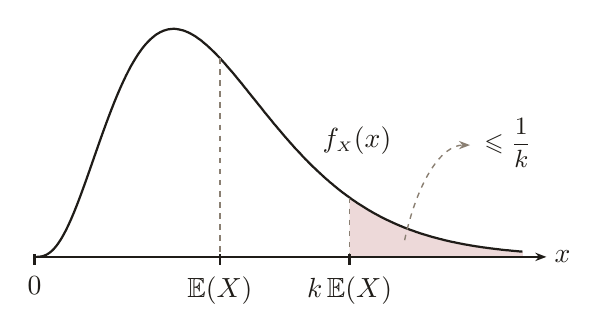
\begin{tikzpicture}[
  x=1cm,
  y=7.6cm,
  every node/.style={font=\normalsize, journalink},
  axis/.style={journalink, line width=0.8pt, -{Stealth[length=4pt]}},
  tick/.style={journalink, line width=0.8pt},
  curve/.style={journalink, line width=0.8pt},
  guide/.style={journalmuted, line width=0.5pt, dash pattern=on 2pt off 2pt},
  pointer/.style={journalmuted, line width=0.5pt,
                  dash pattern=on 2pt off 2pt, -{Stealth[length=4pt]}},
  tail/.style={journalaccent, fill opacity=0.18}
]
  % ---- the right tail [k E(X), 6.2] ------------------------------------
  % Shading path per spec 1.6: from the foot of the left boundary along the
  % x axis to the foot of the right boundary, up to the curve, back along the
  % curve, cycle.
  \fill[tail]
    (4,0) -- (6.2,0) -- (6.2,0.0087772)
    -- plot[domain=6.2:4, samples=200, smooth] (\x,{\gammafour{\x}})
    -- cycle;

  % ---- density curve: Gamma(4, 1.7) ------------------------------------
  \draw[curve] plot[domain=0:6.2, samples=300, smooth] (\x,{\gammafour{\x}});

  % ---- x axis ----------------------------------------------------------
  \draw[axis] (0,0) -- (6.5,0);
  \node[anchor=west, inner sep=2.8pt] at (6.5,0) {$x$};

  % ---- the two boundaries ----------------------------------------------
  \draw[guide] (2.352941,0.3321236) -- (2.352941,0);
  \draw[guide] (4,0.0992252) -- (4,0);
  \foreach \p in {0, 2.352941, 4}
    \draw[tick] ([yshift=0.035cm]\p,0) -- ([yshift=-0.106cm]\p,0);
  % One row of labels: the two boxes are 0.4133cm and 0.5354cm wide either
  % side of their centres, which stand 1.647cm apart, so they clear each other
  % by 0.698cm, above the 0.6cm of spec 1.3.
  \node[anchor=north, inner sep=0pt] at ([yshift=-0.25cm]0,0) {$0$};
  \node[anchor=north, inner sep=0pt] at ([yshift=-0.25cm]2.352941,0)
    {$\mathbb{E}(X)$};
  \node[anchor=north, inner sep=0pt] at ([yshift=-0.25cm]4,0)
    {$k\,\mathbb{E}(X)$};

  % ---- curve label ------------------------------------------------------
  % Bottom left corner (3.65, 1.30cm); the curve stands 1.038cm there, so the
  % box clears it by 0.262cm.
  \node[anchor=south west, inner sep=0pt] at ([yshift=1.30cm]3.65,0)
    {$f_{\sssig X}(x)$};

  % ---- callout from the centroid of the shaded tail ---------------------
  \draw[pointer] ([yshift=0.211776cm]4.699108,0)
    .. controls ([yshift=0.95cm]4.86,0) and ([yshift=1.42cm]5.16,0)
    .. ([yshift=1.42cm]5.53,0);
  \node[anchor=east, inner sep=0pt] at ([yshift=1.45cm]6.32,0)
    {\small $\leqslant\dfrac{1}{k}$};
\end{tikzpicture}
\end{document}
